\label{ch6}
\section{簡介}
由於第\ref{ch4}章,專注式機制對於系統表現有蠻大的幫助。且第\ref{ch5}章中,非監督式學習的語音詞向量,也有小幅的贏過動態時間規劃,若能夠將部分有標注的資料去微調模型,說不定能有更大的進步。所以在此章中,想將第\ref{ch5}章的語音詞向量跟第\ref{ch4}的專注式機制合併,變成半監督式學習法(Semi-Supervised),使用部分標記資料跟部分非標記資料來訓練,希望進而相輔相成,使其效能能夠更進步。
\section{模型架構}
\subsection{模型簡介}
圖\ref{ch6_model}為本章的模型架構圖,其概念是將第\ref{ch4}章跟第\ref{ch5}章的模型做結合,首先語音查詢詞跟語音文件先分別抽出聲學特徵後,經過圖\ref{ch6_att}將一連串聲學特徵轉變為代表查詢詞之向量$V_Q$跟代表語音文件之向量$V_D$,之後經過類神經網路分類器,產生出查詢詞出現在語音文件的機率。同時,模型能夠藉由圖\ref{ch6_a2v},將產生之向量經由解碼器還原成原本聲學序列。

%圖\ref{ch6_model}為本章的模型架構圖,跟第\ref{ch4}章提出的模型相同。同樣地,語音文件跟語音查詢詞都會先從音訊檔案中抽取聲學特徵。接著遞迴類神經網路編碼器將語音查詢詞之聲學特徵轉變成語音查詢詞向量 $ V_Q$,如圖\ref{ch6_att}(A),而語音文件向量則是採用專注式機制,利用語音查詢詞向量$V_Q$跟每個時間點的語音文件去計算餘弦相似度當作專注式權重,最後依照權重得到語音文件向量$V_D$,如圖\ref{ch6_att}(B)所示。得到$V_Q$跟$V_D$後,丟入分類器產生查詢詞出現在文件的機率。
\begin{figure}
\centering
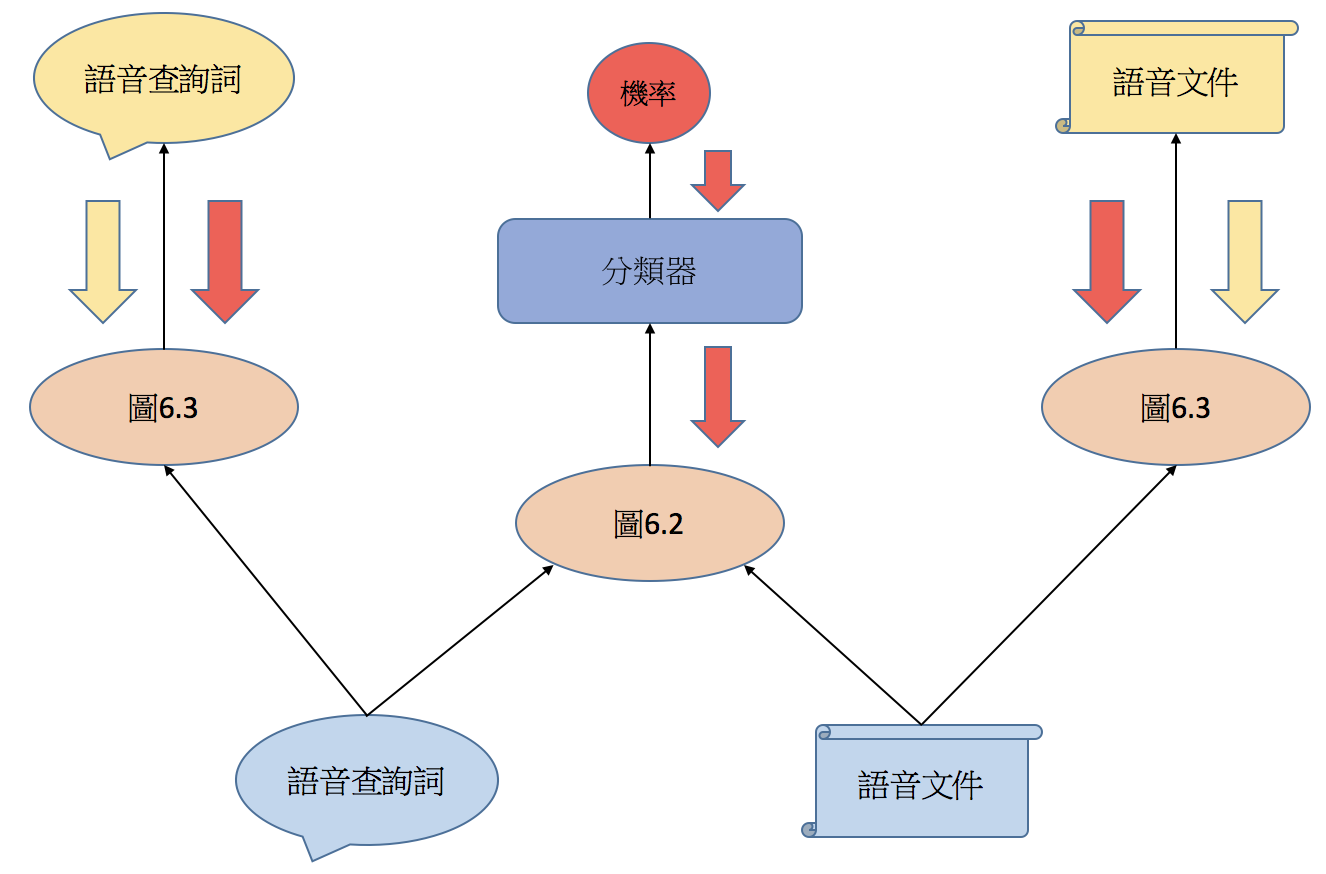
\includegraphics[scale=0.5]{images/ch6_model.png} 
\caption{模型架構圖}
\label{ch6_model}
\end{figure}
圖\ref{ch6_att}為產生查詢詞向量$V_Q$跟語音文件向量$V_D$的方法,第\ref{ch4}章的方法一模一樣,語音查詢詞經過遞迴類神經網路後,取其最後一個時間點當作$V_Q$,藉由$V_Q$與每個時間點遞迴類神經網路的語音文件向量輸出計算餘弦相似度,獲得一長度跟語音文件相同的權重值後,進行加權平均,來得語音文件向量$V_D$。

\begin{figure}
\centering
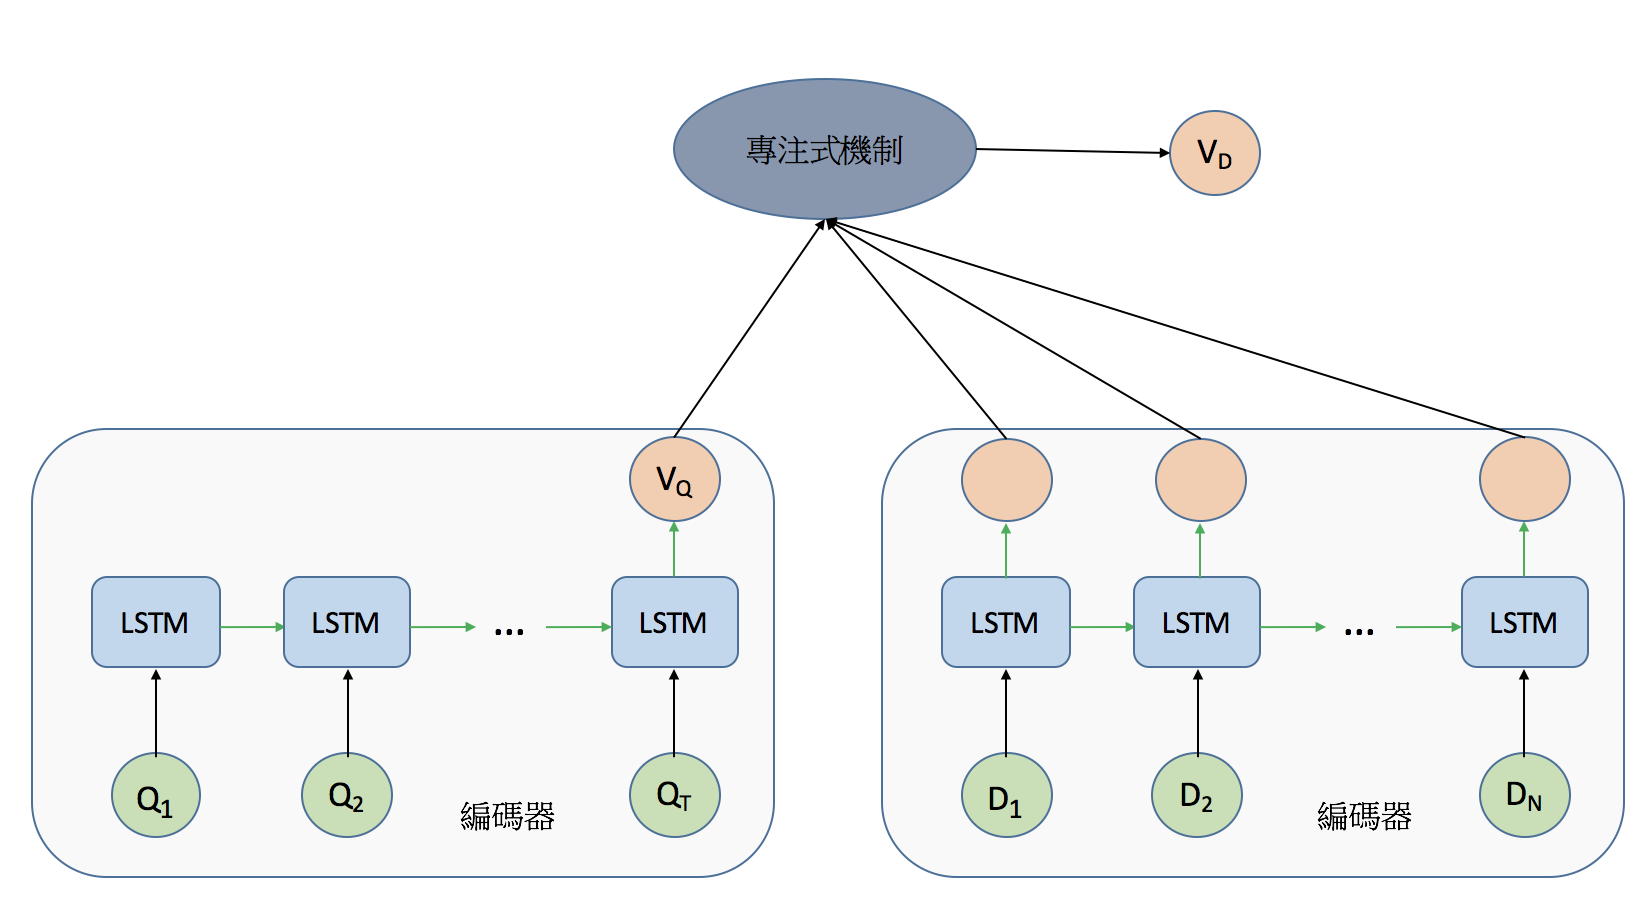
\includegraphics[scale=0.5]{images/ch6_att.png} 
\caption{專注式機制圖}
\label{ch6_att}
\end{figure}
圖\ref{ch6_a2v}為跟第\ref{ch5}章相同的序列對序列模型,將聲學序列經過遞迴類神經網路後產生的隱藏狀態,藉由解碼器轉回原本之聲學序列。此模型在此可以看做一正規化的機制,限制編碼器產生的向量不僅能精準的分類出查詢詞是否出現在語音文件,同時最後的隱藏狀態應該能夠保留著整段聲學序列的資訊。如此模型就不能單純做好分類問題,而必須同時達到其他目標,進而避免模型發生過度貼合之情形。
\begin{figure}
\centering
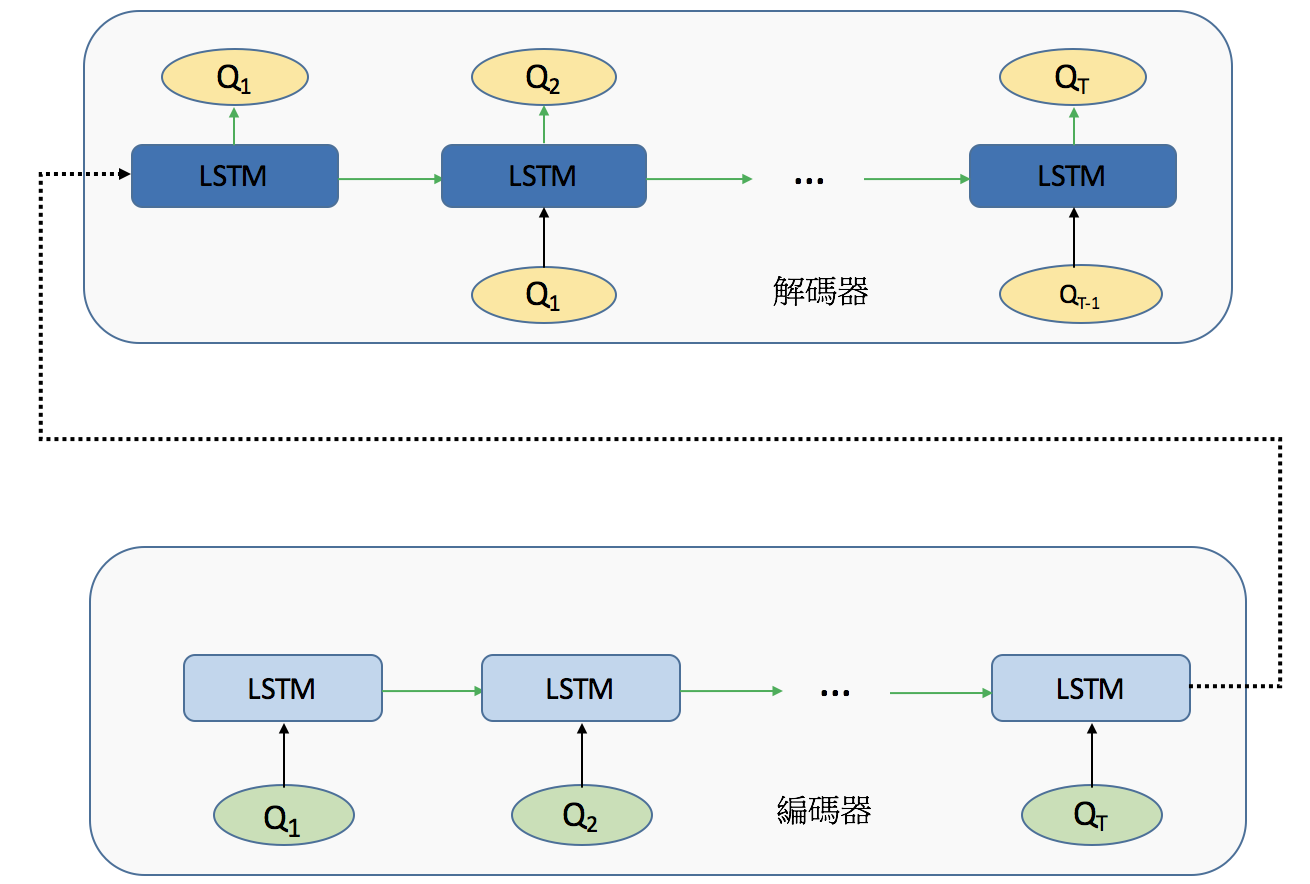
\includegraphics[scale=0.5]{images/ch6_a2v.png} 
\caption{語音詞向量正規化機制圖}
\label{ch6_a2v}
\end{figure}
\subsection{訓練方式}
此時因模型為多任務學習(Multi-Task
Learning),模型需要同時分類正確,且能夠還原成原本的語音序列。其損失函數會對於其任務有所不同,其一為交叉熵如式\ref{eq:ch5_LCE},為了提高口述詞彙偵測的正確率。
\begin{equation}
\label{eq:ch5_LCE}
L_{CE}(\bold{x} , \bold{y} , \theta) =KL(\bold{y} || f_{\theta}(\bold{x}))= KL( \bold{y} ||\hat{\bold {y}} )  = - \log \hat{y}_{l} 
\end{equation}
其中KL為克雷散度,$\bold{y}$為正確答案,$\hat{\bold{y}}$為模型預測之結果,$\hat{y_l}$為模型給正確標籤的分數。
而另一個損失函數為均方根差\ref{eq:ch5_RMSE},使其編碼向量能夠能夠完整還原最初之語音序列。
\begin{equation}
\label{eq:ch5_RMSE}
L_{rmse} (\bold{x},\bold{y}) = \sum_{i=1}^{T}
RMSE(\bold{x}_i-\bold{y}_i) = \sum_{i=1}^{T} \sum_{j=1}^D \sqrt{(x_{ij}-y_{ij})^2}
\end{equation}
其中RMSE為方均根差,$\bold{x}$為輸入之語音序列,$\bold{y}$為模型還原之語音序列,$\bold{x}_i$為時間點$i$之聲學特徵,$\bold{y}_i$
為時間點$i$之模型還原聲學特徵,T為輸入序列長度,D為聲學特徵向量維度。
\section{實驗與分析}
\subsection{實驗設定與基準實驗}
\begin{itemize}
\item{實驗設定}

	訓練語料為LIBRISPEECH 的英語語料,從train-clean-360
	取出30,000個語音文件當作訓練語料,用來訓練語音詞向量;取出70,000筆查詢詞跟語音文件配對,查詢詞共500個,用來訓練分類器。測試語料跟章節\ref{ch4}的設定相同,分成測試集$1$(查詢詞聲學特徵跟訓練語料相同)、測試集$2$(查詢詞聲學特徵跟測試集不同)、測試集$3$(查詢詞未出現在訓練語料)。
	
	在訓練的時候,會先訓練語音詞向量的部分,為監督式學習的部分,如圖\ref{ch6_model}上黃色箭頭的部分。接著才會訓練分類器。而在訓練分類器的同時,也會同時希望能夠還原成初始的語音序列,如圖\ref{ch6_model}上紅色箭頭部分。

\vspace{10cm}
\item{基準實驗}

	基準實驗仍為利用動態時間規劃得到的分數,在分別在測試集$1$得到0.6173的平均準確率,測試集$2$得到0.5778的平均準確率,測試集$3$得到0.5668的平均準確率。
\end{itemize}
\subsection{實驗結果與分析}
表\ref{table:ch6_exp}為本章實驗結果,編碼器為各種層數的長短期記憶網路,每一層有128個神經元。分類器使用四層的類神經網路,其架構為128-64-32-2。可以發現有了標記的資料進行訓練,使模型表現比第\ref{ch5}章的模型跟基準實驗的表現進步許多,然而加上了語音詞向量當作正規化,使模型同時要分類正確並由向量還原初始的語音序列。兩種任務無法達成互補的效果,使其平均準確率較第\ref{ch4}章的模型低了一個層級,不論使用幾層的編碼器,效能仍不及單純的專注式模型。
\begin{table}[ht]
	 \centering
	 \caption{專注式遞迴類神經網路實驗結果}
	 \label{table:ch6_exp}
	 \begin{tabular}{|c|c|c|c|c|}
		 \hline
		 \multicolumn{2}{|c|}{模型架構} & 測試集1 & 測試集2 & 測試集3 \\
		 \hline
		 \multicolumn{2}{|c|}{基準實驗} & 0.6173 & 0.5778 & 0.5678\\
		 \hline
		 \multicolumn{2}{|c|}{專注式模型} & 0.6523 & 0.6246 & 0.5754\\
		 \hline 
		 編碼器模型 & 分類器模型 & 測試集1 &測試集2 & 測試集3 \\
		 \hline
		 一層長短期記憶網路&\multirow{3}{*}{類神經網路} &
		   0.6232 &0.6005 & 0.5674\\
		 \cline{1-1}\cline{3-5}
		 兩層長短期記憶網路& & 0.6358 & 0.6035 & 0.5779 \\
		 \cline{1-1}\cline{3-5}
		 三層長短期記憶網路& & 0.6423 & 0.6104 & 0.5700 \\ 
		 \hline
	   \end{tabular}
\end{table}
\section{本章總結}
本章節將第\ref{ch4}章專注式機制跟第\ref{ch5}章語音詞向量的方法結合,使模型變為多任務學習,同時能夠將口述詞彙精準的找出,並藉由語音詞向量的訓練,使編碼器產生較好的向量表示,然而最後結果多任務學習拖累了原本主要的目的口述詞彙偵測的表現,並無達到相輔相成的效果。
